
\subsection{What is Algebraic Topology}


Recall Metric Spaces: $(X, d)$, $X$ is a set, $d$ is a metric on $X$ (ie. $d: X \times X \to \bR$)
\begin{enumerate}
    \item $d(x,y)=0$ exactly if $x=y$
    \item $d(x,y) = d(y,x)$
    \item $d(x,z) \le d(x,y) + d(y,z)$ 
\end{enumerate}

\noindent
Let $V$ be a vector space, let $|| \cdot ||$ be a norm on $V$, let $d(v,w) = ||v-w||$ 
\begin{itemize}
    \item $\bR^n$: $||(r_j)||_2 = (\Sigma |r_j|^2)^{\frac{1}{2}}$ - Euclidean Norm, $||(r_j)||_1 = \Sigma |r_j|$, $||(r_j)| = \max {|r_j|}$
\end{itemize}

\noindent
If (X,d) is a metric space and if $Y \subseteq X$, let $d^Y$ be the restriction of $d$ to $Y \times Y$. Then $(Y, d^Y)$ is a metric space. \\

\noindent
Metric spaces $\ifff$ geometry: length, area, size of angles. \\

\noindent
Let $X$ be a balloon on $\bR^3$
\begin{itemize}
    \item Two natural metrics: inherited metric from $\bR^3$, path-lenght metric (eg. length of shortest path on surface between two points) 
    \item Consider a deformation: 
    \[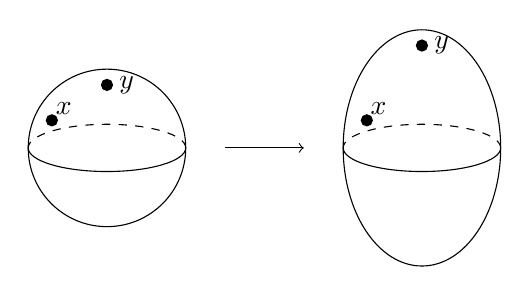
\begin{tikzpicture}
        \draw (-1,0) circle (1cm);
        \draw (-2,0) arc (180:360:1 and 0.3);
        \draw[dashed] (0,0) arc (0:180:1 and 0.3);
        
        \draw[->] (0.5, 0) -- (1.5, 0) ;
        
        \draw (3,0) circle (1cm and 1.5cm);
        \draw (2,0) arc (180:360:1 and 0.3);
        \draw[dashed] (4,0) arc (0:180:1 and 0.3);
        
        \filldraw [black] (-1.7,0.35) circle (2pt);
        \node at (-1.55, 0.5) {$x$};
        
        \filldraw [black] (-1,0.8) circle (2pt);
        \node at (-0.75, 0.8) {$y$};
        
        \filldraw [black] (2.3,0.35) circle (2pt);
        \node at (2.45, 0.5) {$x$};
        
        \filldraw [black] (3,1.3) circle (2pt);
        \node at (3.25, 1.3) {$y$};
      \end{tikzpicture}\]
        the shapes have different Euclidean distances but still have an underlying commonality 
    \item We also observe that the balloon cannot be continuously deformed into the shape below: 
    \[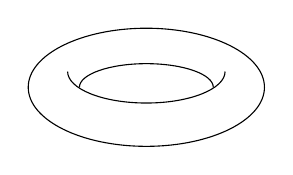
\begin{tikzpicture}
        \draw (0,0) circle (1.5cm and 0.75cm);
        \draw (-1 ,0.2) arc (180:360:1 and 0.4);
        \draw (0.85,0) arc (0:180:0.85 and 0.3);
    \end{tikzpicture}\]
\end{itemize}

\noindent
We want to be able to prove such things without embedding into a metric space. This is done by attaching algebraic objects to topological spaces such that their isomorphism classes dont change under continuous deformation. 

\subsection{Continuity} 

Let $(X, d^X)$ and $(Y, d^Y)$ be two metric spaces. Let $f: X \to Y$ be a function. Let $x_0 \in X$. We say $f$ is continuous at $x_0$ if for all $\ve > 0$ there exists $\delta > 0$ such that if $d^X(x, x_0) < \delta$ then $d^Y(f(x), f(x_0)) < \ve$. 

\begin{itemize}
    \item Let $(X,d)$ be a metric space. By the open ball of radius $r$ about $x_0$, we mean $B(x_0, r) = \{x \in X \, : \, d(x, x_0) <r \}$ (closed ball is $\{x \in X \, : \, d(x, x_0) \le r \}$ )
    \item the above definition can be rephrased as: for any $B(f(x_0), \ve)$ there is an open ball $B(x_0, \delta)$ such that if $x \in B(x_0, \delta)$ then $f(x) \in B(f(x_0), \ve)$. \\
    eg. For every open ball $B_1$ about $f(x_0)$ there is an open ball $B_2$ about $x_0$ such that if $x \in B_2$ then $f(x) \in B_1$ 
\end{itemize}

\begin{definition}
    For $(X,d)$ a metric space, by a neighborhood of a point $x \in X$, we mean any subset of $X$ that contains an open ball about $x$. 
\end{definition}

\begin{itemize}
    \item rephrasing the definition again we get: For any neighborhood $N_{f(x_0)}$ of $f(x_0)$ there is a neighborhood $N_{x_0}$ of $x_0$ such that if $x \in N_{x_0}$ then $f(x) \in N_{f(x_0)}$ 
\end{itemize}

\begin{definition}
    $f: X \to Y$ is continuous if it is continuous at each points of $X$. 
\end{definition}
